%% Week 2 course preprint in IJCAI style. Not submitted to or accepted by IJCAI.
%% Official style: copy ijcai26.sty and named.bst from the IJCAI-ECAI 2026 author kit
%% (https://www.ijcai.org/authors_kit) into this folder. Without them, this file falls
%% back to a plain two-column layout so it still compiles.
\documentclass{article}
\pdfpagewidth=8.5in
\pdfpageheight=11in
\IfFileExists{ijcai26.sty}{\usepackage{ijcai26}}{%
  \usepackage[letterpaper,margin=0.75in,columnsep=0.25in]{geometry}%
  \AtBeginDocument{\twocolumn}}
\usepackage{times}
\IfFileExists{soul.sty}{\usepackage{soul}}{}
\usepackage{url}
\usepackage[hidelinks]{hyperref}
\usepackage[utf8]{inputenc}
\usepackage[small]{caption}
\usepackage{graphicx}
\usepackage{amsmath}
\usepackage{amssymb}
\usepackage{booktabs}
\usepackage{xcolor}
\urlstyle{same}
\providecommand{\affiliations}{\\}
\providecommand{\shortcite}{\cite}
\newcommand{\todo}[1]{\textcolor{red}{\textbf{[TODO: #1]}}}
\newcommand{\hyp}{$^{\dagger}$}
\newcommand{\Pc}{P(\mathrm{C})}

\title{Cloud Cost Agent:\\Which Check Next? A Probabilistic and Information-Theoretic Agent for Unexplained AWS Cost Spikes}
\author{Vaishnavi \affiliations Independent DevOps Engineer, Karnataka, India}

\begin{document}
\maketitle
\renewcommand{\thefootnote}{}\footnotetext{Course preprint (Week 2, AI-Native AI Engineering). Not submitted to or accepted by IJCAI; the IJCAI format is used for style only. Numbers marked \hyp\ are hypothetical assumptions; all results are from simulation.}\renewcommand{\thefootnote}{\arabic{footnote}}

\begin{abstract}
When an AWS cost line item spikes, an operator must decide whether to ignore it, send it to a human, or limit the resource, without seeing the cause. We extend a Week~1 Bayesian agent so that it also decides \emph{which} evidence to buy. The agent holds a belief over five hidden causes, including a residual ``other'' state, measures its uncertainty as entropy, and buys one of four paid checks only when its value of information---the expected saving minus price and delay---is positive. We compare a do-nothing baseline, a most-likely-cause policy, a cost-derived threshold policy, and three value-of-information policies on 20 seeds of 500 simulated cases. The most accurate policy (0.871) costs 4.4 times more than the final agent (\$72,704 vs.\ \$16,648 per 500 cases). The most informative check has the most negative value (0.63 bits, $-$\$2,414), and in only 2 of 600 situations was the most informative check also the best purchase. Three design changes came from failure analysis: losses that depend on the bill size, a residual state, and a stricter guard on automatic limits. When the agent's evidence model is wrong, its advantage over the threshold policy largely disappears (12 of 20 seeds). With one-sided feedback, the agent's learned prior drifts towards ``safe''; a weighted 5\% audit corrects most of the drift.
\end{abstract}

%% =============================================================
\section{Introduction}

A cloud bill rises. The cause might be normal variation, a planned batch job, a forgotten resource (waste), leaked keys running an attacker's workload (compromise), or something else, such as an AWS price change. Each cause calls for a different response, and each wrong response has a different price: ignoring a compromise lets the bill grow, limiting a planned job causes a self-inflicted outage, and reporting everything creates alert fatigue.

Asking a large language model ``is this a hack?'' is not enough. It returns an answer without a calibrated probability, without the cost of each mistake, and without any way to decide whether a \$1 lookup or a \$2,000 investigation is worth doing first. The agent needs (i)~a \emph{belief} over causes, (ii)~\emph{costs} to turn belief into action, and (iii)~a rule for \emph{which information to buy}.

In Week~1 the agent observed one daily line item and chose ignore, investigate, limit, or report. This paper keeps that problem and asks:

\begin{quote}\emph{When an AWS cost line item spikes, which check should the agent run next, and at what belief should it stop checking and act?}\end{quote}

\paragraph{The same equation as an umbrella.} With a 35\% chance of rain, I would leave the umbrella on a walk (carrying it costs 3 units, getting wet costs 6; break-even $3/6=0.50$), but take it to a client demo with my laptop (getting wet costs 400; break-even $3/400=0.0075$). The probability is the same; the consequences decide. My agent's threshold for reporting a possible compromise is the same equation (Section~\ref{sec:policy}).

\paragraph{Contributions.} (1)~A five-state belief model with eight evidence sources, four of which have a price and a delay. (2)~A value-of-information policy with an explicit stop rule. (3)~An experiment with six policies, a misspecified simulator, generalization tests, a Jensen--Shannon shift alarm, and a study of one-sided feedback. (4)~Eight classified failures and three design changes, each re-tested. Code: \url{https://github.com/Vaishnavi1607678/Cloud-Cost-Agent}.

%% =============================================================
\section{Related Work}

I did not read new research papers this week, and I cite none rather than list papers I have not read. The two ideas this paper builds on, that information has value only if it can change a decision, and that unequal error costs should change a decision rule, are standard in decision theory; reading the original sources is part of my next step. The concepts in Section~\ref{sec:info} were learned with AI-assistant explanations and checked by computing them on my own model. Two of them, selection bias in feedback and conditional independence, I looked for because of my own results (Sections~\ref{sec:results} and~\ref{sec:fail}).

%% =============================================================
\section{The Probabilistic View}
\label{sec:prob}

\paragraph{Observation.} One daily line item: service, region, usage, cost, the previous 7 days, and the bill amount (\$1 to \$1,165/day in the main sample, median \$68).

\paragraph{Hidden states and priors.} Normal 0.78, Planned 0.08, Waste 0.07, Compromise 0.03, Other 0.04\hyp. These are judgements: the Week~1 prior with four points moved to a new residual state, because Week~1 failure analysis showed that price changes were mistaken for spikes.

\paragraph{Evidence.} Free: spike level (today vs.\ 7-day median: \emph{low} $<1.5\times$, \emph{med} $<3\times$, \emph{high} $\geq 3\times$), price jump (cost up, usage flat), new region, owner tag (\$0.01). Paid: CloudTrail launcher (\$1, 1 min), change ticket (\$5, 5 min), asking the owning team (\$40, 2 h), security forensics (\$2,000, 48 h). Only one likelihood is measured: P(spike level $\mid$ Normal) $=(0.67, 0.21, 0.12)$, from 115 unmodified service-days in the Week~1 billing data. All other likelihoods are judgements\hyp, e.g.\ P(high $\mid$ Compromise) $=0.75$, P(untagged $\mid$ Compromise) $=0.85$, P(known launcher $\mid$ Compromise) $=0.30$ (stolen keys show a real user).

\paragraph{Posterior.} By Bayes' rule, $P(s \mid e) = P(e \mid s)P(s) / \sum_{s'} P(e \mid s')P(s')$. Table~\ref{tab:bayes} shows the first update by hand: after a high spike, compromise rises from 3\% to 12.4\%, although 75\% of compromises cause a high spike. Confusing $P(e\mid s)$ with $P(s\mid e)$ is exactly the error Bayes' rule prevents.

\begin{table}[t]\centering\small
\begin{tabular}{lrrrr}\toprule
State & Prior & $P(\text{high}\mid s)$ & Product & Posterior\\\midrule
Normal & 0.78 & 0.12 & 0.0936 & 0.517\\
Planned & 0.08 & 0.45 & 0.0360 & 0.199\\
Waste & 0.07 & 0.30 & 0.0210 & 0.116\\
Compromise & 0.03 & 0.75 & 0.0225 & 0.124\\
Other & 0.04 & 0.20 & 0.0080 & 0.044\\\midrule
Sum & 1.00 & & 0.1811 & 1.000\\\bottomrule
\end{tabular}
\caption{One Bayes update by hand (spike $=$ high).}\label{tab:bayes}
\end{table}

\paragraph{Belief-state table.} Table~\ref{tab:belief} follows one example through all free evidence. Entropy rises twice: after the high spike (1.177 $\rightarrow$ 1.889 bits) and after ``untagged'' (1.613 $\rightarrow$ 1.996 bits). The agent knows more but is more confused: it has moved from ``probably normal'' to ``something is happening, but I don't know what''. Expected information gain is never negative, but the gain from a single outcome can be.

\begin{table}[t]\centering\small\setlength{\tabcolsep}{3.5pt}
\begin{tabular}{lrrrrrr}\toprule
Evidence & N & P & W & C & O & $H$ (bits)\\\midrule
prior & .780 & .080 & .070 & .030 & .040 & 1.177\\
spike high & .517 & .199 & .116 & .124 & .044 & 1.889\\
no price jump & .523 & .212 & .124 & .133 & .007 & 1.777\\
region seen & .574 & .233 & .136 & .049 & .009 & 1.613\\
untagged & .293 & .179 & .313 & .211 & .005 & 1.996\\\bottomrule
\end{tabular}
\caption{Belief-state table for one example\hyp. Implied action: Report (expected cost \$162.8, vs.\ Ignore \$1,179.9 and Limit \$397.2).}\label{tab:belief}
\end{table}

%% =============================================================
\section{The Information-Theoretic View}
\label{sec:info}

I include only the concepts the agent uses, each with one number from this problem.

\textbf{Entropy} is the agent's confusion in bits: 1.177 at the prior, out of a maximum of $\log_2 5 = 2.32$. \textbf{Information gain}, which is the same quantity as \textbf{mutual information} $I(S;E)$, is the expected drop in entropy after a check. At the prior, the spike signal is worth 0.171 bits and the owner tag 0.091 bits. \textbf{Conditional entropy} $H(S\mid\text{spike}) = 1.006$ bits is the confusion expected to remain. Unlike correlation, mutual information works on categories and on any shape of dependence.

\textbf{KL divergence} measures how badly one belief describes a world that follows another. It is not symmetric: for the belief of Table~\ref{tab:belief}, $D(\text{post}\,\|\,\text{prior}) = 1.047$ bits but $D(\text{prior}\,\|\,\text{post}) = 0.898$ bits, so it is not a distance. If the world contains a 4\% ``Other'' state and the agent has none, $D(\text{world}\,\|\,\text{agent})$ is infinite. \textbf{Jensen--Shannon divergence} compares both beliefs to their average; it is symmetric and finite (0.020 bits in that case), which makes it usable as an alarm (Section~\ref{sec:results}). \textbf{Cross-entropy} (log loss) is the average surprise at the truth; it rises from 0.778 to 1.473 bits when the residual state is removed. \textbf{Calibration} asks whether the agent's 30\% means 30\%.

\textbf{Value of information} (VOI) turns bits into money:
\begin{equation}
\begin{split}
\mathrm{VOI}(e) ={}& \min_a \mathbb{E}[c(a,S)] \\
& - \Big(\textstyle\sum_o P(o)\min_a \mathbb{E}[c(a,S)\mid o] \\
& \quad + \text{price}_e + \text{delay}_e\Big),
\end{split}
\end{equation}
where $\text{delay}_e$ is the check's duration times the expected hourly loss of an unhandled problem. If no outcome can change the action, the bracket equals the first term plus price, so VOI is negative.

%% =============================================================
\section{Information Selection}

Table~\ref{tab:evidence} compares the four paid checks at the belief of Table~\ref{tab:belief}. Ranked by bits, forensics is first; ranked by value, it is last by far. The CloudTrail check carries fewer bits than every other check but gives the most value per dollar (20.7 bits per \$100) and the highest VOI.

\begin{table}[t]\centering\small\setlength{\tabcolsep}{3pt}
\begin{tabular}{lrrrrr}\toprule
Check & IG (bits) & Price & Time & Bits/\$100 & VOI\\\midrule
launcher & 0.244 & \$1 & 1 min & 20.72 & \textbf{+\$55.0}\\
ticket & 0.274 & \$5 & 5 min & 4.65 & $-$\$5.9\\
ask owner & 0.522 & \$40 & 2 h & 0.85 & +\$13.3\\
forensics & \textbf{0.628} & \$2,000 & 48 h & 0.03 & $-$\$2,414\\\bottomrule
\end{tabular}
\caption{Evidence comparison at the belief of Table~\ref{tab:belief} (\$60/day)\hyp. Bits/\$100 counts price plus expected delay loss.}\label{tab:evidence}
\end{table}

\paragraph{Five candidate questions.} At the prior, the agent's five questions (owner tag, launcher, ticket, ask the owner, forensics) carry 0.091, 0.063, 0.136, 0.191 and 0.152 bits, but only the \$0.01 owner tag has positive VOI (+\$2.3), so it is always read. The others are bought only after the free evidence has made the agent uncertain. The policy in four sentences: \emph{read the four free signals; recompute the belief; buy the paid check with the most bits per dollar among those whose VOI is positive; repeat until no check has positive VOI.}

\paragraph{Is the most informative question always best?} No. In the case of Table~\ref{tab:evidence}, forensics could change the action, but saves far less than its \$2,000 price plus about \$513 of expected loss while waiting 48 hours. I then searched 600 situations (every free-evidence combination $\times$ 5 investigation histories $\times$ 5 bill sizes): the most informative remaining check was also the best purchase with positive value in only \textbf{2} (0.3\%). In both, the belief was split between Normal (0.652) and Planned (0.250), and the change ticket, the one check that separates exactly those two, was the most informative (0.316 bits) and worth buying, by only \$3.22. \emph{Rule: information has value only if an outcome can change the action, and only if that change saves more than the check costs.}

%% =============================================================
\section{Decision Policy}
\label{sec:policy}

\paragraph{Actions and costs.} Ignore, Report (send to a human), or Limit. At a \$60/day line item, costs\hyp\ are as in Week~1: Ignore costs \$400 for Waste, \$5,000 for Compromise, \$100 for Other; Report costs \$50 (\$600 for Compromise); Limit costs \$300 for Normal, \$1,500 for Planned, \$100 for Compromise. From failure FW2-1, the loss from ignoring a problem depends on the bill $A$: Waste $6.67A$ (spend runs about a week), Compromise $\$3{,}200 + 30A$ (fixed incident cost plus a month of attacker spend), Other $1.67A$.

\paragraph{Derived thresholds.} Report beats Ignore for a possible compromise when $\Pc > 50/(50+4{,}400) = 1.1\%$ at \$60/day; at \$1,000/day it is 0.15\%. Limit beats Report when $\Pc > 250/(250+500) = 33\%$ if the alternative is Normal, but 74\% if it is Planned. The cheap middle action, Report, is what makes a 1\% threshold usable.

\paragraph{Escalation.} A human decides (Report) when the belief is in the uncertain band, when an automatic Limit would apply below $\Pc = 0.7$ (design change DC3), or whenever the bill exceeds \$3,000/day, whatever the confidence. Report is also the default safe action.

\paragraph{Stop rule.} Stop buying when no remaining check has positive VOI, when two checks in a row move the belief by less than 0.02 (total variation), or after four paid checks.

%% =============================================================
\section{Experiment}

\paragraph{Simulation.} For each case, the true state is drawn from the prior and every evidence outcome from the likelihood tables. The bill amount is a real row of the Week~1 data multiplied by a factor matching the spike level ($0.5$--$1.5$, $1.5$--$3$, $3$--$10$). The main run uses 500 cases at seed 42; robustness uses 20 seeds (100--119). Every policy sees identical cases, and labels are read only after all decisions. A \emph{misspecified} simulator breaks two assumptions: stolen keys show a known launcher 60\% of the time (the agent assumes 30\%), and, for normal and planned work, ``untagged'' and ``unknown launcher'' come together (automation roles), which the agent treats as independent.

\paragraph{Policies.} P0: always Ignore. P1: act on the most probable state after free evidence. P2: lowest expected cost after free evidence. P3: P2 plus value-of-information checks and the stop rule. P3b: P3 with bill-dependent costs (DC1). P3c: P3b with the 0.7 Limit guard (DC3), the final agent.

\paragraph{Metrics.} Accuracy (the action is the cheapest for the true state), precision and recall for problems (Waste or Compromise vs.\ Report or Limit), total cost (decision $+$ check prices $+$ delay losses), checks per case, human-review rate, cross-entropy, and expected calibration error (ECE).

%% =============================================================
\section{Results}
\label{sec:results}

\begin{table}[t]\centering\small\setlength{\tabcolsep}{3pt}
\begin{tabular}{lrrrrrr}\toprule
 & P0 & P1 & P2 & P3 & P3b & P3c\\\midrule
Accuracy & .861 & \textbf{.871} & .590 & .685 & .673 & .672\\
Recall & .000 & .531 & \textbf{.952} & .897 & .849 & .849\\
False pos. & 0 & 34.1 & 203.5 & 155.9 & 158.2 & 158.2\\
Missed C & 15.25 & 3.05 & 0.00 & 0.05 & 0.10 & 0.10\\
Wrong Limit & 0.00 & 1.50 & 0.70 & 1.15 & 1.15 & 1.05\\
Total (k\$) & 235.2 & 72.7 & 19.3 & 18.2 & \textbf{16.4} & 16.6\\
Checks/case & 0 & 0 & 0 & 0.52 & 0.28 & 0.28\\
Human \% & 0 & 10.0 & 49.0 & 37.7 & 37.6 & 37.8\\
ECE & .010 & .019 & .019 & .018 & .018 & .018\\\bottomrule
\end{tabular}
\caption{Mean over 20 seeds $\times$ 500 cases, matched simulator. False positives, missed compromises, and wrong Limits are counts per 500 cases.}\label{tab:main}
\end{table}

\begin{figure}[t]\centering
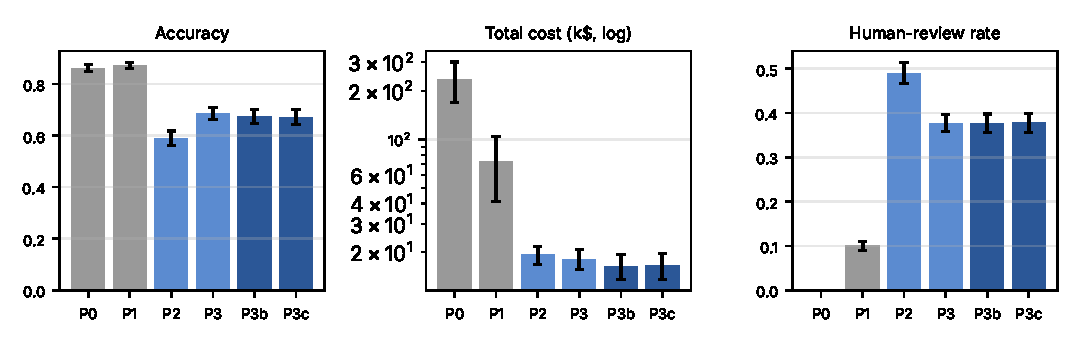
\includegraphics[width=\columnwidth]{figures/fig1_policies.pdf}
\caption{Accuracy, total cost (log scale), and human-review rate per policy (20 seeds, error bars = 1 s.d.). The most accurate policies are the most expensive.}\label{fig:policies}
\end{figure}

\paragraph{Accuracy is the wrong headline.} P1 is the most accurate policy and costs 4.4 times more than P3c (Table~\ref{tab:main}, Figure~\ref{fig:policies}). It rarely flags anything, so it is usually right and occasionally very expensive. P2 is the least accurate and is already close to the best cost. Buying checks (P3) lowers human review from 49\% to 38\% and cost by about 6\%. Making costs depend on the bill (P3b) lowers cost again, to \$16,409, and halves the number of checks.

\paragraph{When the model is wrong.} In the misspecified simulator, P3 becomes \emph{worse} than P2 (\$23,236 vs.\ \$19,433): it buys the CloudTrail check, double-counts it with ``untagged'', and wrongly limits 5.8 normal workloads per 500 cases instead of 1.2. Here, more information made decisions worse. The final P3c costs \$19,278 and beats P2 in only 12 of 20 seeds (19 of 20 in the matched world). ECE rises from 0.018 to 0.024.

\paragraph{Generalization.} I changed one variable at a time (P3b, 20 seeds):
(a)~\emph{Missed-problem cost $\times 100$:} the Report threshold falls from 0.0112 to 0.0001, and human review rises to 95.6\% (P2: 98.5\%). The agent now verifies almost everything, so human review capacity, not the model, becomes the limit.
(b)~\emph{Checks cost $\times 10$:} checks per case fall from 0.28 to 0.12; cost rises only from \$16,409 to \$16,876, still below P2's \$19,313. The agent shifts from asking to reporting.
(c)~\emph{Unreliable history (startup $\rightarrow$ enterprise):} in an enterprise world\hyp\ (more planned jobs and attacks, 99\% of normal resources tagged, 25\% of normal launchers unknown automation roles), the stale startup model costs \$21,578 vs.\ \$19,725 when re-fitted, a 9\% penalty for not knowing the world changed. The best evidence also changes: a missing tag becomes much stronger evidence of compromise in the enterprise world, while an unknown launcher becomes weaker. Portable: the cost-derived threshold, the VOI rule, and the stop rule. Local: every prior and likelihood.

\begin{figure}[t]\centering
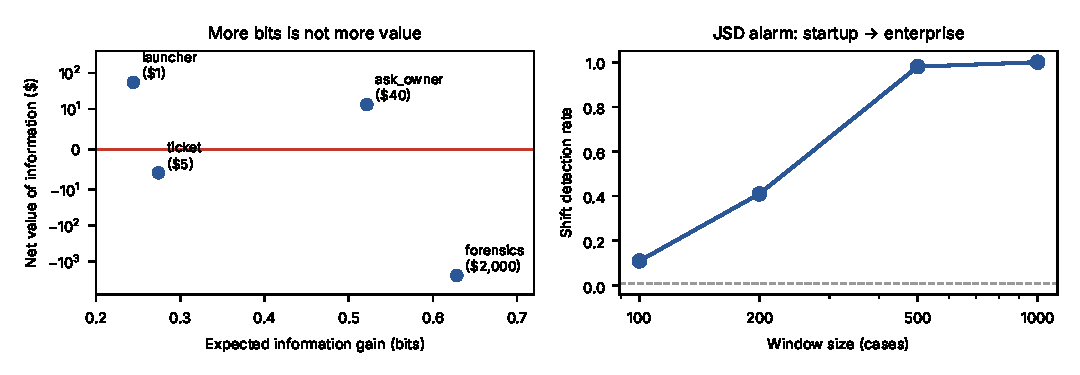
\includegraphics[width=\columnwidth]{figures/fig2_information.pdf}
\caption{Left: information gain vs.\ net value of information for the four paid checks (belief of Table~\ref{tab:belief}). Right: JSD alarm detection rate for the startup$\rightarrow$enterprise shift by window size (false-alarm rate fixed at 1\%).}\label{fig:info}
\end{figure}

\paragraph{Noticing the shift.} The agent compares the distribution of the 24 free-evidence patterns in a window with a 5,000-case startup reference using JSD, with an alarm level at the 99th percentile of startup windows. Detection is 11\% with 100-case windows, 41\% with 200, 98\% with 500, and 100\% with 1,000 (Figure~\ref{fig:info}), all at a 1\% false-alarm rate. The shift is visible before any labels arrive, but only with enough cases.

\paragraph{Feedback.} If the agent learns its prior from feedback but ignored cases produce no complaint and are counted as Normal, its estimate of P(Waste) after 5,000 cases is 0.100 when the truth is 0.12, and more data does not fix it. Full feedback gives 0.120. Auditing a random 5\% of ignored cases and weighting each by $1/0.05$ (inverse-probability weighting) gives 0.117 and cuts $D(\text{world}\,\|\,\text{learned prior})$ from 0.0154 to 0.0025 bits. In this setting the biased prior barely changes total cost, because P2 decides mostly from evidence. The harm is a picture of the world that is wrong and does not correct itself.

%% =============================================================
\section{Failure Analysis}
\label{sec:fail}

P3 made 146 wrong decisions on the main 500 cases. I analysed the most expensive ones with the brief's ten questions (full answers in \texttt{results/failure-analysis.md}).

\textbf{FW2-1 Forgotten planned job} (\$3,362; \emph{wrong cost assumption}). A \$509/day waste case was ignored at belief Planned 0.726: a change ticket existed, for a job that was never shut down. The evidence was true but misleading, and the agent assumed every bill was \$60, so ignoring waste looked like a \$400 risk instead of \$3,395. \emph{DC1:} losses depend on the bill. Re-test: this case is now reported; mean cost \$18,152 $\rightarrow$ \$16,409, lower in 18 of 20 seeds; recall fell from 0.897 to 0.849.

\textbf{FW2-2 Price change ignored} (\$216; \emph{wrong cost assumption}). The residual state raised Other to 0.17, but a fixed \$100 cost made ignoring cheaper than reporting. Fixed by DC1.

\textbf{FW2-3 Untagged normal work looks like an attack} (\$301; \emph{misleading evidence}). Untagged, new region, unknown launcher: $\Pc = 0.658$, Limit. The two clues share one cause, so naive Bayes counts it twice. \emph{DC3:} Limit guard 0.5 $\rightarrow$ 0.7. Re-test: misspecified wrong Limits 5.85 $\rightarrow$ 3.80 and cost \$19,655 $\rightarrow$ \$19,278; matched cost +\$239. A 0.9 guard removes almost all wrong Limits (0.30) but adds about \$2,200, because real compromises then go to a human. I chose 0.7, the guard with the lowest worst-case cost across both worlds.

\textbf{FW2-4 Stolen keys look like a known user} (\$502; \emph{misleading evidence}). A known launcher pulled $\Pc$ down to 0.081, so the agent reported instead of limiting. Not changed: I need real data, not a guess tuned to my simulator.

\textbf{FW2-5 Quiet compromise} (\$500; \emph{insufficient information}). A compromise with a medium spike: $\Pc = 0.042$. Asking the owner would have exposed it, but no answer could change Report to Limit at that belief, so its VOI was negative. Report was the right safe default.

\textbf{FW2-6 Slow leak} (\$519; \emph{bad evidence}). Waste with a low spike: nothing looked wrong. No evidence source in my model can see it; it needs a utilisation signal.

\textbf{FW2-7 Insurance reporting} (113 cases; \emph{wrong cost assumption}). Most errors are normal spikes sent to a human at \$50 each, because the threshold is 1.1\%. If a report really costs more (alert fatigue), the threshold rises; Week~1's sensitivity test showed false alarms falling from 14.2 to 3.2 per 40 cases at \$150.

\textbf{FW2-8 Missing residual state} (\emph{missing hidden state}). Without ``Other'', cost rises from \$16,409 to \$16,861 (worse in 15 of 20 seeds) and cross-entropy from 0.778 to 1.473 bits. \emph{DC2:} keep the residual state.

%% =============================================================
\section{Human Discussions}

At the time of writing, no human discussion had changed my understanding of the problem: the Week~2 questions had not yet been answered. I report this rather than leave the section out. The questions I am asking this week come from my failures: how often stolen keys appear as a known CloudTrail user (FW2-4), whether practitioners would allow an automatic stop of an untagged resource (FW2-3), how long waste runs before it is noticed (the $6.67A$ assumption), and whether teams audit the alerts they did not raise (feedback bias).

%% =============================================================
\section{Limitations}

\textbf{Data:} the only data is 30 days of mock billing rows; only the Normal spike likelihood and the typical \$60 bill are measured. \textbf{Simulation:} cases are generated from my own likelihood tables, so the main experiment validates the \emph{policy} given those likelihoods, not the likelihoods. The misspecified simulator shows how much the result depends on them. \textbf{Assumed probabilities:} all priors and all other likelihoods. \textbf{Assumed costs:} every cost, including how long waste and attacks run and the \$50 cost of a Report, which ignores alert fatigue. \textbf{Suspected missing states:} a planned job that turned into waste (FW2-1), and insider misuse. \textbf{Independence:} naive Bayes double-counts linked clues (FW2-3). \textbf{Generalization:} priors and likelihoods are local to one account type. \textbf{Human oversight:} every automatic Limit should still be approvable by a human in deployment; the agent never deletes anything.

%% =============================================================
\section{New Questions}

(1)~\emph{Can the agent learn which clues are linked from its own decision log, without being told, and stop double-counting them?} (FW2-3.) (2)~\emph{What audit rate is enough to keep a learning agent's prior honest when feedback only arrives for flagged cases, and does the answer depend on how rare the dangerous state is?} (3)~\emph{When the JSD alarm fires, what should the agent do during the 500 cases it needs to be sure: fall back to P2, widen the Report band, or raise the Limit guard?}

%% =============================================================
\section*{AI-Use Statement}
I used Claude (Anthropic) to explain the Week~2 concepts in simple language, to write and debug the Python model, simulator, and experiments, to compute the tables, and to draft this paper's LaTeX and the appendix answers. The hidden states, the evidence sources, and the cost assumptions were designed in conversation with the assistant and are my responsibility. The assistant ran the experiments in its workspace from the code in the repository; every number in this paper comes from those scripts (seeds 42 and 100--119) and can be reproduced with the commands in the README. The assistant found and fixed two of its own errors during the work (an unrealistic cost scaling and an incorrect audit weighting).

\section*{Contribution Statement}
Single author, with AI assistance as described above.



%% =============================================================
\appendix
\onecolumn
\section{Required Core Questions}

\begin{enumerate}\small
\item \textbf{Hidden state.} Something true that the agent cannot see but that decides the right action. Mine: Normal, Planned, Waste, Compromise, Other.
\item \textbf{Why direct prediction is not enough.} A single answer (``compromise'') hides how sure it is and ignores costs. At 12\% compromise the right action is still Report, which a yes/no prediction cannot express.
\item \textbf{Belief distribution.} A probability for every hidden state. It must sum to one because the states are meant to cover every possibility exactly once; the residual ``Other'' state takes whatever my list misses.
\item \textbf{Prior vs.\ posterior.} Prior: belief before the evidence (compromise 0.03). Posterior: belief after it (0.124 after a high spike).
\item \textbf{Likelihood.} How probable the evidence is if a state were true: P(high spike $\mid$ compromise) $=0.75$. Probability of the state given the evidence is different: P(compromise $\mid$ high spike) $=0.124$.
\item \textbf{Uncertainty.} Probability spread over several states. My agent at Table~\ref{tab:belief} gives Waste 0.31, Normal 0.29, Compromise 0.21, Planned 0.18.
\item \textbf{Entropy.} The average number of yes/no questions needed to find the true state; it is highest when all states are equally likely. Prior: 1.177 bits; after free evidence: 1.996 bits.
\item \textbf{Bit.} The information in one fair yes/no answer.
\item \textbf{Information gain.} Expected entropy before minus expected entropy after a check: CloudTrail gives 0.244 bits at Table~\ref{tab:belief}.
\item \textbf{Conditional entropy.} The uncertainty expected to remain after seeing a signal: $H(S \mid \text{spike}) = 1.006$ bits.
\item \textbf{Mutual information vs.\ correlation.} Mutual information measures any dependence, including between categories, as reduced uncertainty: $I(S;\text{spike}) = 0.171$ bits. Correlation only measures straight-line relations between numbers.
\item \textbf{KL divergence.} The extra surprise from using belief $Q$ when the world follows $P$. Not a distance, because it is not symmetric and does not satisfy the triangle inequality.
\item \textbf{KL asymmetry.} $D(\text{post}\|\text{prior}) = 1.047$ but $D(\text{prior}\|\text{post}) = 0.898$ bits. If the world has a 4\% ``Other'' state and the agent has none, one direction is infinite and the other is 0.059 bits.
\item \textbf{Jensen--Shannon divergence.} The average KL of two distributions to their mixture: symmetric and always finite (0 to 1 bit), so it can compare evidence patterns even when one window has zero counts. My shift alarm uses it.
\item \textbf{Calibration.} Stated probabilities match observed frequencies. If the agent's 30\% is really 60\%, its expected-cost decisions are wrong. ECE: 0.018 (matched) vs.\ 0.024 (misspecified).
\item \textbf{Expected cost and my threshold.} Probability-weighted cost of an action. Report beats Ignore when $50 < 4{,}400 \times P(\mathrm{C})$, i.e.\ above 1.1\%.
\item \textbf{Value of information.} The expected saving from a check minus its price and delay. More information is not worth it when no answer can change the action, or when the saving is smaller than the cost: forensics, $-$\$2,414.
\item \textbf{Informative but useless.} Forensics: 0.628 bits, the most informative check, and the worst purchase at Table~\ref{tab:belief}.
\item \textbf{Distribution shift and detection.} The world changes but the agent's priors do not. My agent compares free-evidence patterns with a reference using JSD; 500-case windows detect a startup$\rightarrow$enterprise shift 98\% of the time at a 1\% false-alarm rate.
\item \textbf{Stop rule.} Stop when no remaining check has positive value of information, when two checks in a row barely move the belief, or after four checks; then act on the lowest expected cost, and send to a human if the action is a Limit below 0.7 or the bill is over \$3,000/day.
\end{enumerate}

\end{document}
